\documentclass[11pt,letterpaper,twocolumn]{article}
\usepackage[margin=0.75in]{geometry}
\usepackage[T1]{fontenc}
\usepackage{lmodern}
\usepackage{amsmath,amssymb}
\usepackage{graphicx}
\usepackage{booktabs}
\IfFileExists{placeins.sty}{\usepackage{placeins}}{}
\usepackage{float}
\IfFileExists{balance.sty}{\usepackage{balance}}{}
\usepackage{setspace}
\setstretch{1.12}
\raggedbottom
\usepackage[numbers,sort&compress]{natbib}
\usepackage[bookmarks=false]{hyperref}
\usepackage[font=small,labelfont=bf]{caption}
\usepackage{xcolor}

\graphicspath{{figures/}{./}}

\setlength{\columnsep}{0.30in}
\setlength{\parskip}{0.35em}
\setlength{\parindent}{1em}
\renewcommand{\arraystretch}{1.03}
\setlength{\textfloatsep}{15pt plus 3pt minus 3pt}
\setlength{\floatsep}{12pt plus 3pt minus 2pt}
\setlength{\intextsep}{12pt plus 3pt minus 2pt}
\setlength{\emergencystretch}{1.5em}

\setcounter{topnumber}{4}
\setcounter{bottomnumber}{2}
\setcounter{totalnumber}{6}
\renewcommand{\topfraction}{0.95}
\renewcommand{\bottomfraction}{0.85}
\renewcommand{\textfraction}{0.05}
\renewcommand{\floatpagefraction}{0.80}
\setcounter{dbltopnumber}{2}
\renewcommand{\dbltopfraction}{0.95}
\renewcommand{\dblfloatpagefraction}{0.80}

\renewenvironment{abstract}{%
  \section*{\abstractname}\vspace{-0.25em}
}{\par\vspace{0.6em}}

\hypersetup{colorlinks=true, linkcolor=black, citecolor=black, urlcolor=black}


\newcommand{\added}[1]{#1}
\usepackage{tikz}
\usetikzlibrary{arrows.meta,positioning}
\definecolor{seqblue}{HTML}{135E96}
\definecolor{ctxgreen}{HTML}{239DAD}
\definecolor{fusionpurple}{HTML}{168BC4}
\newcommand{\figureplan}[2]{\fbox{\parbox[c][42mm][c]{0.93\linewidth}{\centering\small
\textbf{Figure assembly pending: #1}\\[4pt]#2\\[4pt]
\footnotesize Panel specifications and source paths: FIGURE\_GUIDE.md}}}

\title{\LARGE\bfseries SilentMethyl predicts CpG methylation and local variant effects using sequence and chromatin context}
\author{%
  Samuel Zhang$^{1,2}$, Shaojun Pei$^{1,2,*}$, and Gil Alterovitz$^{1,2,*}$ \\[0.5em]
  \small $^{1}$Division of General Internal Medicine and Primary Care, \\
  \small Brigham and Women's Hospital, Boston, Massachusetts, United States \\
  \small $^{2}$Harvard Medical School, Harvard University, Boston, Massachusetts, United States \\[0.5em]
  \small $^{*}$Authors for correspondence: \href{mailto:spei1@bwh.harvard.edu}{spei1@bwh.harvard.edu} (Shaojun Pei); \\
  \small \href{mailto:gil\_alterovitz@hms.harvard.edu}{gil\_alterovitz@hms.harvard.edu} (Gil Alterovitz)
}
\renewcommand{\thepage}{\arabic{page}}
\date{}


\begin{document}
\maketitle
\begin{abstract}
DNA methylation is a key component of epigenetic regulation, yet predicting how individual variants alter it remains challenging. Here, we present SilentMethyl, a gated fusion model integrating DNA sequence with reference breast epigenomic context. On 26,570 chromosome-held-out CpGs, fusion achieves beta-value mean absolute error 0.0914 and ROC-AUC 0.974, improving on individual modalities and retrained methylation architectures. Independent breast and blood mQTLs and allele-specific methylation support modest agreement with predicted variant effects. Distance matching reduces blood mQTL discrimination from AUROC 0.600 to 0.556. Despite improving baseline accuracy, fusion adds little variant-effect signal over sequence alone. Gate decomposition shows that fixed context can modulate allelic differences without substantially improving external agreement. Transfer errors concentrate at tissue-variable CpGs, while synonymous and nonsynonymous case studies illustrate experimental prioritization. SilentMethyl distinguishes accurate methylation prediction from allelic inference and provides a framework for evaluating local regulatory hypotheses.
\end{abstract}

\section{Introduction}
DNA methylation is a widely studied epigenetic modification involved in gene regulation, shown to be associated with genomic context, chromatin organization, and transcription \cite{jones2012functions,schubeler2015function}, and frequently dysregulated in disease. Single-nucleotide variants (SNVs) can influence local epigenetic states, but validating their direct regulatory effects is difficult because matched genetic and epigenetic data are limited. This motivates modeling DNA methylation to identify potentially functional variants.

Existing deep learning methods have been able to predict DNA methylation and other regulatory measures using local DNA sequence, neighboring methylation, and long-range sequence context \cite{angermueller2017deepcpg,zhou2015predicting,avsec2021effective}. While DNA sequence itself contains motifs and local regulatory patterns, sequence alone misses the epigenetic context in which they operate. Reference epigenomic data, including chromatin accessibility, histone modifications, and evolutionary conservation, can account for some of this missing information. Predicting methylation at a single locus and estimating the effect of a base change on methylation are also distinct tasks. A model that accurately predicts baseline methylation may still estimate variant-induced changes poorly.

Several frameworks for evaluating paired sequence changes already exist. CpGenie predicts CpG methylation and validates REF--ALT sequence changes against methylation quantitative trait loci (mQTLs) \cite{zeng2017cpgenie}. INTERACT focuses on methylation in brain tissue, DeepMethylation/DDM combines DNA sequence with reference tissue data, and Metheven combines sequence with ATAC-seq chromatin accessibility \cite{zhou2022interact,li2026deepmethylation,liu2025methven}. More recently, Melody extends sequence-based methylation prediction across multiple cell types \cite{jin2026melody}. These approaches establish sequence-based methylation modeling as a route to regulatory interpretation, while differing in the information available to each model and the biological question being evaluated.

Because these studies use different tissue types, model targets, sequence windows and data splits, their reported metrics do not provide a common benchmark. Comparisons must distinguish the prediction of an existing methylation state from the prediction of its response to an allele change. Reference chromatin can improve the former without necessarily providing additional information about the latter. Similarly, variants close to a CpG may be easier to identify as methylation-associated than more distant variants. An evaluation that does not control for this proximity can overstate how much discrimination comes from the sequence model itself.

SilentMethyl was designed to examine these questions within one framework. It combines a pretrained DNA sequence encoder with a reference-context multilayer perceptron (MLP) through learned gates. We compare the fused model with its individual modalities and with methylation architectures retrained on the same data. Reverse-complement augmentation during training and orientation averaging during inference address strand dependence \cite{mallet2021rc}. We then evaluate paired REF--ALT predictions against independent mQTL and allele-specific methylation (ASM) data, separating agreement in direction and rank from discrimination between associated and control variants.

SilentMethyl also uses synonymous mutations as a focused application for variant prioritization, since they modify a base pair without changing the encoded amino acid. However, synonymous SNVs can still affect local regulatory function, including splice recognition, RNA structure, transcript stability, translation, and regulatory sequences in exons \cite{sauna2011understanding,stergachis2013exonic}. Published examples link synonymous variants in \textit{MLH1}, \textit{TP53}, and \textit{ADAMTS13} with methylation-associated phenomena or altered CpG content \cite{alvarez2025mlh1,blackburn2016tp53,jankowska2022adamts13}. These examples motivate examining effects beyond altered protein sequence, without implying that all synonymous variants share a methylation mechanism. A computational screen can identify specific variant--CpG pairs for study, while separating a predicted local response from the broader functional consequences of the same substitution. We retain a synonymous \textit{NCOA2} case study and extend the same scoring procedure to nonsynonymous \textit{STK11} variants, while distinguishing these hypotheses from external validation.

Here, we show that integrating sequence and primary breast-epithelium context improves CpG methylation prediction across held-out chromosomes. Independent cohorts support modest agreement with predicted allelic changes, but better baseline prediction does not translate into a clear variant-effect advantage over sequence alone. A within-model decomposition explains how context enters the allelic contrast, and tissue-transfer analyses identify where prediction becomes less reliable. Together, these analyses define the capabilities and limitations of using multimodal methylation models to prioritize local regulatory variants.

\section{Results}
\subsection{Multimodal fusion improves methylation prediction}
\label{sec:performance}
SilentMethyl integrates a 1,000-bp CpG-centered sequence with reference epigenomic information through gated fusion (Fig.~\ref{fig:silentmethyl_workflow}). The sequence tower uses DNABERT-2 followed by convolution and attention pooling. The context tower encodes seven primary breast-epithelium chromatin measurements and two conservation scores, together with missingness indicators. The resulting representations are combined to predict a continuous methylation value and a binary methylation state. Paired allele substitutions are scored using the same trained model and reference context, allowing baseline accuracy and predicted variant responses to be evaluated separately.

Methylation targets were constructed from 97 TCGA-BRCA solid-tissue-normal samples, with each CpG represented by the median of its observed beta values. The retained dataset contained 418,486 unmasked CpGs. Chromosome-level partitioning assigned 345,359 loci to training, 46,557 to validation, and 26,570 to testing. This design prevents neighboring sequence windows on the same chromosome from crossing between training and evaluation partitions. Because the target is a cohort median, the evaluation measures variation across genomic loci rather than variation among individual patients.

Results were obtained on the 26,570-probe test set. The fusion model had the strongest performance across the reported evaluation metrics and seeds. The lightweight context MLP established a beta mean absolute error (MAE) of 0.1022 and receiver operating characteristic area under the curve (ROC-AUC) of 0.9658. Sequence alone reached beta MAE $0.1099\pm0.0008$ and ROC-AUC $0.9569\pm0.0007$. Fusion reduced MAE to $0.0914\pm0.0037$ and raised ROC-AUC to $0.9744\pm0.0025$, a 16.8\% reduction in mean error relative to sequence alone (Fig.~\ref{fig:performance}a). The reported dispersions describe variation across three training seeds.

The comparison with additional baselines supported the same conclusion. Composition and reverse-complement-collapsed $k$-mer ridge models had beta MAEs of 0.1954 and 0.1565. CpGenie and the DNA module of DeepCpG, retrained on identical splits, reached 0.1281 and 0.1253, respectively (Supplementary Table~S1). Both exceeded the classical baselines, but neither matched the sequence or fusion models. Because DNABERT-2 has a larger pretrained encoder, these results compare complete modeling strategies; they do not isolate an advantage attributable to gated fusion or transformer architecture alone.

The regression task also retained information beyond the binary methylation call. Fusion reached $M$-value MAE $1.0971\pm0.0192$, compared with $1.1941\pm0.0070$ for sequence alone and $1.4574\pm0.0023$ for context alone. The two endpoints therefore answer related but different questions: classification measures separation around the methylation threshold, whereas continuous error measures how closely the predicted state matches the target. Their joint improvement supports the use of both tasks in evaluation rather than describing a high ROC-AUC as sufficient evidence of accurate methylation values.

\begin{figure*}[t]
\centering
\IfFileExists{figures/workflow.pdf}{\includegraphics[width=\textwidth]{figures/workflow.pdf}}{\IfFileExists{figures/workflow.tikz}{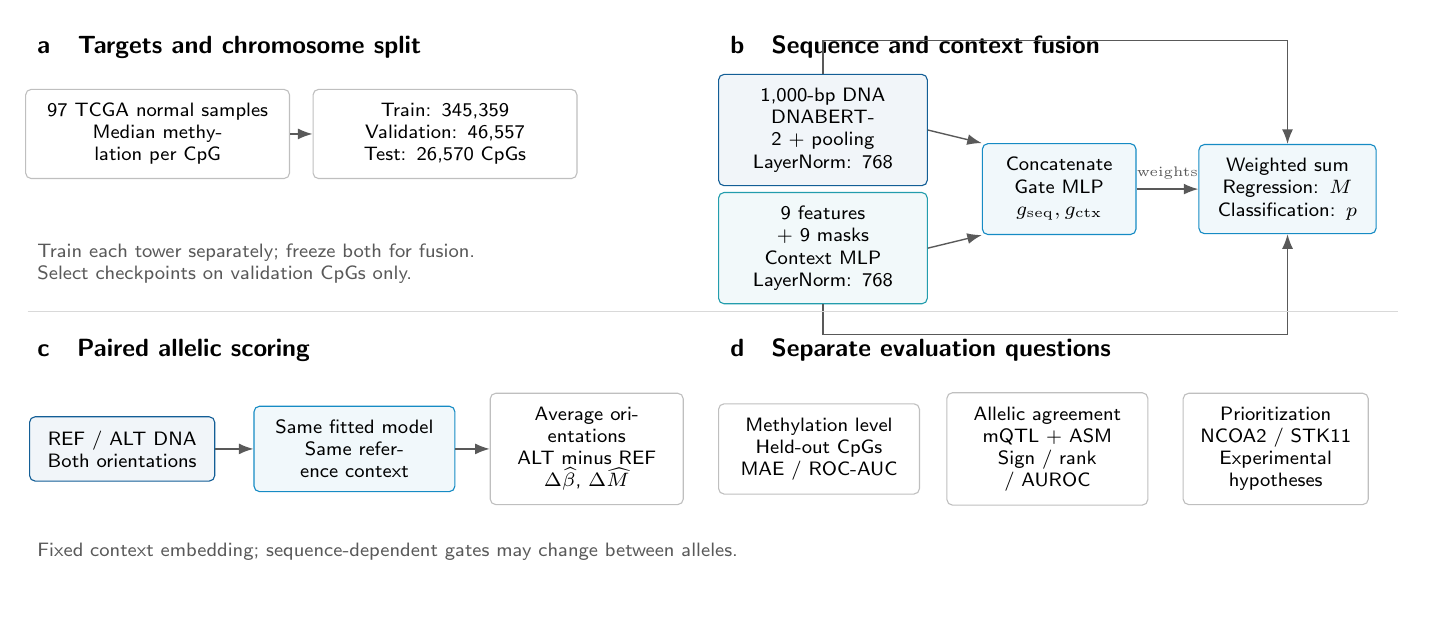
\begin{tikzpicture}[x=1cm,y=1cm,>=Latex,font=\sffamily\scriptsize,
 box/.style={draw=black!25,rounded corners=2pt,align=center,inner sep=5pt},
 seq/.style={box,draw=seqblue,fill=seqblue!6},ctx/.style={box,draw=ctxgreen,fill=ctxgreen!6},fus/.style={box,draw=fusionpurple,fill=fusionpurple!6},arr/.style={->,line width=.5pt,black!65}]
\path[use as bounding box] (0,0) rectangle (17.5,7.25);
\node[anchor=west,font=\sffamily\bfseries\small] at (0,7.0) {a\quad Targets and chromosome split};
\node[box,text width=3.0cm] (target) at (1.65,5.9) {97 TCGA normal samples\\Median methylation per CpG};
\node[box,text width=3.0cm] (split) at (5.3,5.9) {Train: 345,359\\Validation: 46,557\\Test: 26,570 CpGs};
\draw[arr] (target)--(split);
\node[anchor=west,font=\sffamily\bfseries\small] at (8.8,7.0) {b\quad Sequence and context fusion};
\node[seq,text width=2.3cm] (seq) at (10.1,5.95) {1,000-bp DNA\\DNABERT-2 + pooling\\LayerNorm: 768};
\node[ctx,text width=2.3cm] (ctx) at (10.1,4.45) {9 features + 9 masks\\Context MLP\\LayerNorm: 768};
\node[fus,text width=1.6cm] (gate) at (13.1,5.2) {Concatenate\\Gate MLP\\$g_{\rm seq},g_{\rm ctx}$};
\node[fus,text width=1.9cm] (sum) at (16,5.2) {Weighted sum\\Regression: $M$\\Classification: $p$};
\draw[arr] (seq.east)--(gate.north west);\draw[arr] (ctx.east)--(gate.south west);
\draw[arr] (gate)--node[above,font=\tiny]{weights}(sum);
\draw[arr] (seq.north) -- ++(0,.42) -| (sum.north);\draw[arr] (ctx.south) -- ++(0,-.38) -| (sum.south);
\node[anchor=west,align=left,text=black!65] at (0,4.25) {Train each tower separately; freeze both for fusion.\\Select checkpoints on validation CpGs only.};
\draw[black!15] (0,3.65)--(17.4,3.65);
\node[anchor=west,font=\sffamily\bfseries\small] at (0,3.15) {c\quad Paired allelic scoring};
\node[seq,text width=2.0cm] (alleles) at (1.2,1.9) {REF / ALT DNA\\Both orientations};
\node[fus,text width=2.2cm] (shared) at (4.15,1.9) {Same fitted model\\Same reference context};
\node[box,text width=2.1cm] (delta) at (7.1,1.9) {Average orientations\\ALT minus REF\\$\Delta\widehat\beta$, $\Delta\widehat M$};
\draw[arr] (alleles)--(shared);\draw[arr] (shared)--(delta);
\node[anchor=west,font=\sffamily\bfseries\small] at (8.8,3.15) {d\quad Separate evaluation questions};
\node[box,text width=2.2cm] at (10.05,1.9) {Methylation level\\Held-out CpGs\\MAE / ROC-AUC};
\node[box,text width=2.2cm] at (12.95,1.9) {Allelic agreement\\mQTL + ASM\\Sign / rank / AUROC};
\node[box,text width=2.0cm] at (15.85,1.9) {Prioritization\\NCOA2 / STK11\\Experimental hypotheses};
\node[anchor=west,text=black!65] at (0,.6) {Fixed context embedding; sequence-dependent gates may change between alleles.};
\end{tikzpicture}
}{\figureplan{workflow}{Targets, sequence/context towers and paired allelic evaluation}}}
\caption{\textbf{SilentMethyl separates methylation-level prediction from variant-effect evaluation.}
\textbf{a}, Cohort-median methylation targets and chromosome partitions.
\textbf{b}, Sequence and reference-context towers are trained separately, then frozen for fusion training. Layer-normalized embeddings enter both the gate and the weighted sum.
\textbf{c}, REF and ALT use the same context. Predictions are averaged over forward and reverse-complement orientations before subtraction.
\textbf{d}, Held-out level prediction, external allelic evaluation and candidate prioritization answer separate questions.}
\label{fig:silentmethyl_workflow}
\end{figure*}

\subsection{Reference context helps across regulatory environments}
The fusion model's improvement was not confined to one chromosome partition. In three additional seed-42 evaluations, fusion achieved beta MAEs of 0.0873, 0.0934 and 0.0862 on chromosomes 12/18, 4/20 and 13/15/21, respectively, improving on the corresponding sequence tower in each split (Fig.~\ref{fig:performance}b). The test sets contained approximately the same number of probes as the original chr8--9 set. These repeated partitions test sensitivity to the choice of held-out chromosomes within the same underlying cohort; they are distinct from replication in an independent biological dataset. The comparison is paired within each split, so each fusion model is assessed against the sequence tower trained for that partition. Holding the training seed fixed for the additional splits makes their role different from the original three-seed analysis, which measures sensitivity to training initialization on the published chromosome split.

Stratified biological and epigenomic groups showed additional patterns in sequence-to-fusion improvement. Fusion reduced beta MAE across the evaluated genomic-region, CpG-island and chromatin strata. The largest relative gains were observed in the highest ATAC-seq and H3K27ac quartiles, where error decreased by 22.4\% and 22.9\%, respectively (Fig.~\ref{fig:performance}c). These results indicate that reference information can provide complementary evidence at accessible, active regulatory loci, where a sequence-only model may be less able to recover the methylation value.

Absolute and relative improvements nevertheless describe different features of this result. CpG shores showed a larger absolute reduction than islands, but their sequence-only error was also higher. Relative reductions were 17.3\% at shores and 18.4\% at islands. High H3K27me3 showed the smallest relative gain among the reported strata, 10.3\%, compared with 23.9\% in the lowest quartile. Context therefore does not help equally in every regulatory environment, and a high starting error does not necessarily imply a large proportional rescue by fusion.

We also examined two possible sources of apparently strong held-out performance. Only four test windows had a nearest-training 31-mer Jaccard similarity above 0.5, and excluding common-SNP-flagged probes left reported fusion MAE unchanged. These checks reduce concerns about close sequence duplication and a specific class of probe artifacts. They do not exclude every form of memorization, measurement bias or genotype-associated array interference; the chromosome splits and quality controls address complementary aspects of evaluation.

\subsection{Transfer errors concentrate at tissue-variable CpGs}
To assess transfer beyond a breast-trained sequence--methylation relationship, we trained a model on colon, kidney and lung while excluding breast from both training and checkpoint selection. Probes were allocated to individual tissues so that the same sequence was not assigned conflicting training targets. On the same 26,570 held-out breast CpGs, this model achieved beta MAE 0.0978 and ROC-AUC 0.9693. Its MAE was 0.0064 higher than the three-seed breast-trained fusion mean, while the reported sequence-arm transfer penalty was 0.0013.

This modest average penalty concealed substantial differences among loci. Error correlated with measured cross-tissue methylation variance at $\rho=0.488$ and remained associated after controlling for mean methylation (partial $\rho=0.475$). MAE increased from 0.045 in the lowest variance decile to 0.197 in the highest (Fig.~\ref{fig:performance}d). The worst-predicted decile contained more CpG shores than the full test set, 34.8\% versus 24.2\%, and fewer islands, 21.1\% versus 31.0\%. These loci also showed higher H3K4me1/H3K27me3 and lower H3K4me3/accessibility signals.

The pattern locates transfer difficulty at CpGs whose measured methylation differs more strongly across tissues. It does not imply that tissue identity resides entirely in chromatin or that sequence-based regulation is tissue-independent. The comparison also changes the training composition and uses one held-out-tissue seed against a three-seed breast reference mean. Separately, learned gate share did not reliably track cross-tissue variability after adjustment for methylation level (partial $\rho=-0.061$). Gate weights alone therefore do not identify tissue-variable loci or supply direct biological attribution.

\begin{figure*}[t]
\centering
\IfFileExists{figures/fig2_prediction_transfer.pdf}{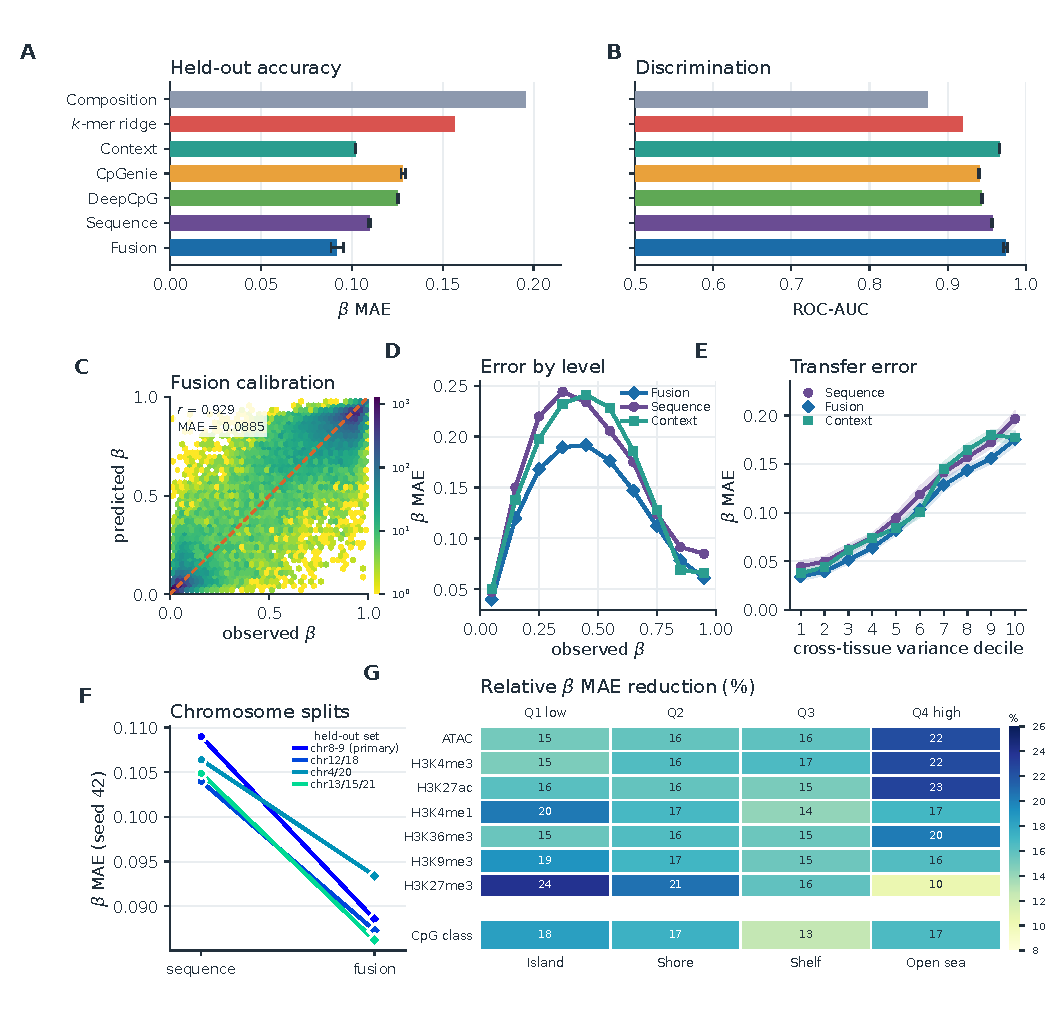
\includegraphics[width=\textwidth]{figures/fig2_prediction_transfer.pdf}}{\figureplan{prediction and transfer}{a Model accuracy\quad b Repeated splits\\c Relative fusion gain\quad d Transfer-error deciles}}
\caption{\textbf{Context improves methylation-level prediction, while tissue variability limits transfer.}
\textbf{a}, Held-out $\beta$ MAE and ROC-AUC, showing individual seeds for stochastic models.
\textbf{b}, Sequence and fusion MAE within each chromosome split at seed 42.
\textbf{c}, Relative MAE reduction, $100(\mathrm{MAE}_{\rm seq}-\mathrm{MAE}_{\rm fusion})/\mathrm{MAE}_{\rm seq}$, by chromatin and CpG-island category; intervals use 2,000 resamples of 1-Mb blocks.
\textbf{d}, Error of the breast-held-out model across cross-tissue methylation-variance deciles. Raw fold and stratum values belong in Source Data.}
\label{fig:performance}
\end{figure*}

\subsection{Independent mQTLs support predicted allelic responses}
To test whether predicted variant-associated methylation differences agreed with external data, we evaluated the breast-trained models in tissue-matched eGTEx breast and GENOA African American whole-blood cohorts. The harmonized held-out sets contained 76,893 and 66,495 variant--CpG pairs, respectively. Primary signed analyses excluded variants that created or destroyed a CpG and used the significant associations in each cohort: 418 breast pairs and 4,037 GENOA pairs. Reference and alternate alleles were aligned before comparison, so predicted and measured directions represented the same substitution.

In the cross-cohort synthesis, fusion achieved signed Spearman correlation 0.236 (95\% confidence interval 0.098--0.392) in breast and 0.149 (0.112--0.185) in GENOA. Direction agreement was 59.6\% (54.2--65.1\%) and 55.6\% (53.8--57.2\%), respectively (Fig.~\ref{fig:external}a). Both cohorts therefore supported modest agreement, with higher point estimates in the tissue-matched analysis. Signed correlation preserves the ordering of negative and positive responses, while direction agreement discards their magnitude and asks only whether the sign is correct. A model can perform differently on these endpoints, particularly when many measured effects are small. Neither metric alone determines how well the model selects variants from a mixture of associated and control pairs. Because tissue, ancestry and cohort design differ together, this comparison cannot attribute the difference specifically to tissue matching or ancestry. Nor do the reported effects share a common biological scale that would justify direct magnitude calibration.

Agreement depended on the strength of the measured association. In GENOA, the signed correlation and direction agreement approached chance among pairs with $p>0.5$, reaching $\rho=-0.004$ and 49.7\% direction agreement. Stronger associations showed clearer correspondence, and agreement was generally better for variants near their target CpG than near the edge of the input window (Fig.~\ref{fig:external}c). High-$p$ pairs are useful benchmark controls, although lack of significance does not establish absence of a biological effect. This qualification is especially relevant when comparing cohorts with different sample sizes.

The 81 independent breast lead-mQTL associations from 70 variants provided a focused positive control, retained from the original analysis. On this selected set, predicted sign separated positive from negative observed slopes at directional AUROC 0.872 (0.780--0.947). Absolute predicted changes agreed more weakly with absolute reported effects: Spearman $\rho=0.217$ with an interval spanning zero. In 35 matched significant/high-$q$ lead pairs, effect magnitude yielded discrimination AUROC 0.512 and permutation $p=0.43$. Thus, good directional ranking among selected lead associations did not establish that large predictions identify significant mQTLs generally.

\subsection{Distance controls limit apparent variant discrimination}
Variant--CpG distance was an important confound in the GENOA benchmark. Distance alone separated significant from tested-but-null pairs at AUROC 0.595 (0.583--0.609), close to the unmatched fusion AUROC of 0.600 (0.586--0.615). Significant associations were, on average, closer to the scored CpG than control pairs. A model could therefore obtain much of its apparent discrimination by responding to proximity, even without correctly ranking effects among variants at similar distances.

After distance matching, fusion retained AUROC 0.556 (0.539--0.572), whereas the position-blind $k$-mer ridge reached 0.5063 (0.4930--0.5191; Fig.~\ref{fig:external}b). This result supports a modest predictive signal beyond the matched proximity distribution and simple sequence composition. The reduction from unmatched to matched performance is itself informative: the larger marginal AUROC should not be read as an independent measure of allele-specific regulatory prediction.

Retrained CpGenie and DeepCpG recovered similar external signal. On a shared matched GENOA cohort, fusion exceeded DeepCpG by 0.019 AUROC (0.005--0.033); its difference from CpGenie was 0.005 ($-0.013$--0.021). Stronger baseline methylation accuracy therefore did not translate into consistently stronger discrimination of methylation-associated variants. The comparison favors reporting model differences on the same matched rows, because changing the negative set can affect marginal AUROC. It also distinguishes residual sequence-model signal from a claim that SilentMethyl uniquely captures that signal.

\subsection{Allele-specific methylation provides a complementary test}
ASM measures methylation separately on the two alleles within heterozygous samples, providing a complementary assessment of a paired-sequence prediction. The Do--Tycko analysis averaged predicted changes over each index SNP's scored differentially methylated region (DMR) CpGs and compared the resulting SNP-level score with the reported allelic difference. This produced 722 evaluable SNPs, including 328 with positive observed effects, with confidence intervals resampling 179 genomic blocks.

Fusion achieved direction agreement 0.590 (0.550--0.630), signed Spearman correlation 0.241 (0.180--0.299), and directional AUROC 0.628 (0.584--0.669). Direction agreement exceeded chance but fell below the prospectively recorded expectation of 0.60--0.70. Correlation and directional AUROC fell within their recorded expectation bands. These are three summaries of the same signed agreement, not independent replications. Sequence-only point estimates were slightly higher on all three measures, without demonstrating a meaningful advantage over fusion (Fig.~\ref{fig:external}d).

Discrimination between ASM and control loci was also above chance in two independently assembled catalogues. Fusion AUROC was 0.5625 (0.533--0.593) in Rosenski--Dor--Kaplan and 0.5419 (0.508--0.580) in Do--Tycko; sequence-only values were 0.5736 and 0.5432. Distance-only baselines were near chance in both. The catalogues use different controls, so their estimates should remain separate rather than be treated as measurements of an identical endpoint. The mammary-only signed subset contained 53 SNPs and did not separate from chance.

A post-hoc restriction to measured effects of at least 20 percentage points increased fusion direction agreement to 0.6055. This is consistent with more direction errors among small observed effects, but it does not replace the primary result or its missed expectation. ASM also extends scoring to genomic CpGs beyond HM450 positions. Consequently, it tests both an allelic contrast and transfer beyond the array's training-position distribution; it does not by itself establish accurate effects at arbitrary breast CpGs.

\begin{figure*}[t]
\centering
\IfFileExists{figures/fig3_external_validation.pdf}{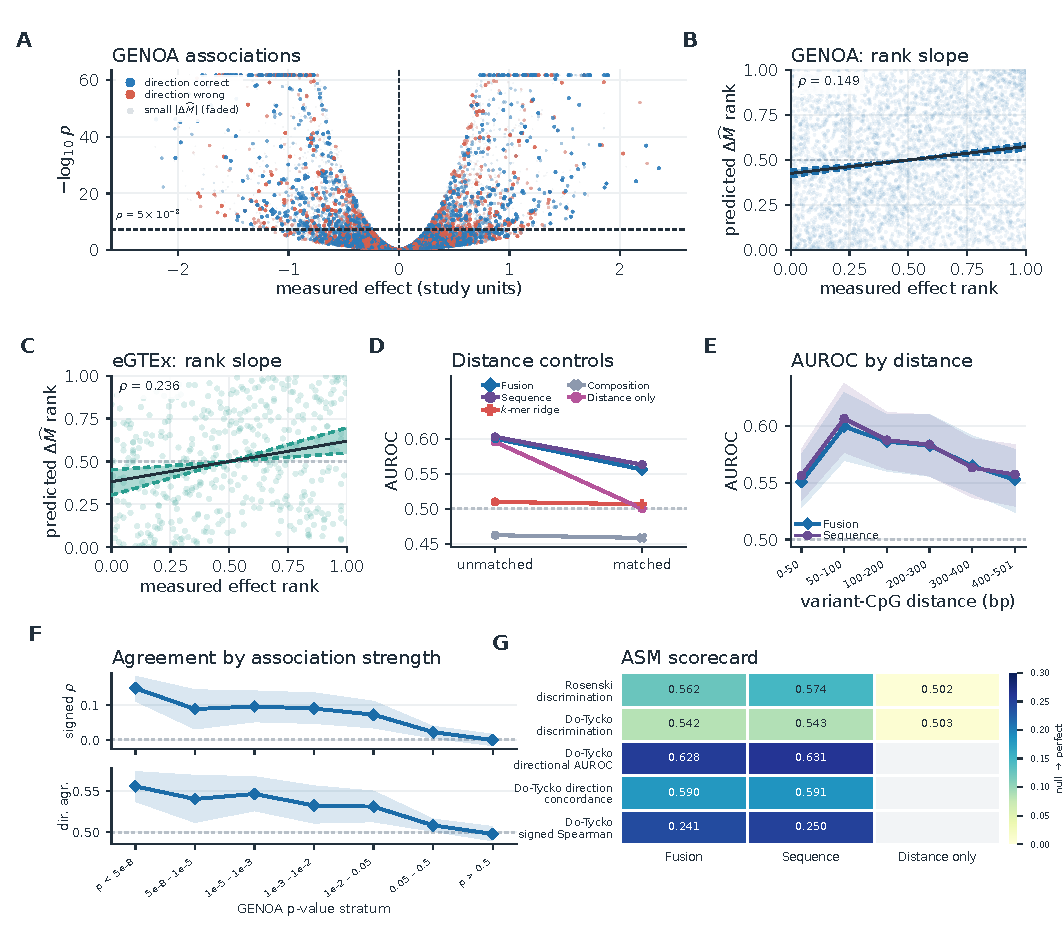
\includegraphics[width=\textwidth]{figures/fig3_external_validation.pdf}}{\figureplan{external allelic evaluation}{a Cohort agreement\quad b Matched discrimination\\c Association-strength gradient\quad d ASM validation}}
\caption{\textbf{External allelic agreement survives explicit benchmark controls.}
\textbf{a}, Signed Spearman correlation and direction agreement in significant breast and GENOA pairs.
\textbf{b}, Unmatched and distance-matched GENOA discrimination, with distance-only and sequence-model controls.
\textbf{c}, GENOA agreement across reported association-strength strata.
\textbf{d}, ASM discrimination in two catalogues and signed agreement in the Do--Tycko set. Each endpoint has its own null reference: zero for correlation and 0.5 for AUROC or direction agreement. Error bars are 95\% genomic-block bootstrap intervals; sample sizes and resampling counts are specified in Methods and Supplementary Table~S2.}
\label{fig:external}
\end{figure*}

\subsection{Context modulates effects with little added external signal}
The sequence-only and fusion models agreed closely in external variant evaluation despite their different baseline accuracies. In the reported paired comparison, fusion-minus-sequence differences were $-0.0010$ ($-0.0078$--0.0051) for signed correlation, 0.0017 ($-0.0050$--0.0079) for direction agreement, and $-0.0023$ ($-0.0058$--0.0010) for distance-matched AUROC (Fig.~\ref{fig:context}a). These intervals show no clear improvement under the evaluated conditions. They constrain the size of a possible gain in this benchmark without proving equivalence in every tissue or variant class.

To understand this result, we separated the contribution of sequence changes from changes in the fusion gates. REF and ALT receive the same context vector, but the gate reads both sequence and context and can change when the allele changes. We therefore evaluated ordered counterfactual inputs to the same fitted regression head: first changing the sequence embedding with gates fixed at REF, then changing the sequence gate, and finally changing the context gate. The resulting components sum to the full predicted effect even when the regression head is nonlinear (Fig.~\ref{fig:context}b).

The decomposition reproduced the total within $2\times10^{-7}$ across 143,388 scored pairs. The gate channel's variance relative to total-effect variance was 18.7\% in GENOA and 19.5\% in eGTEx. Splitting this channel further showed that sequence-gate rescaling dominated, while the context-rescaling component had approximately 6\% of total-effect variance. These ratios do not sum to one because the channels covary. They quantify model behavior under the chosen counterfactual order, rather than uniquely attributing biological effects to separate modalities (Fig.~\ref{fig:context}c).

The distinction between variance and predictive information was substantial. In the cohort-wide GENOA decomposition, the sequence channel alone reached signed correlation 0.0699 with measured effects, compared with 0.0707 for the full contrast. Controlling for the sequence channel left gate-channel partial correlations of 0.0152 (0.0066--0.0247) in GENOA and 0.0091 (0.0017--0.0160) in eGTEx. Context therefore contributes to the numerical contrast, but adds little independent agreement with the measured effects. These cohort-wide correlations use a broader set than the significant-only validation above.

Input perturbations supported a limited contribution, although the conclusion depended on the metric. After normalizing deviations by the unperturbed quantity's standard deviation, shuffling context changed methylation levels more than variant effects, 0.5260 versus 0.2266. Median replacement gave 0.3530 versus 0.1860 (Fig.~\ref{fig:context}d). The original Pearson-based criterion failed for median replacement and is retained in Supplementary Table~S3. Correlation can remain high for broad differences between low- and high-methylation loci even when individual predictions move. Normalized deviation instead describes the size of that movement relative to the original spread. Reporting both avoids replacing an unsuccessful pre-specified comparison with a more favorable metric after inspecting the result. Fixed reference context is therefore neither irrelevant nor guaranteed to improve variant prediction: its contribution must be measured against external allelic outcomes.

\begin{figure*}[t]
\centering
\IfFileExists{figures/fig4_context_mechanism.pdf}{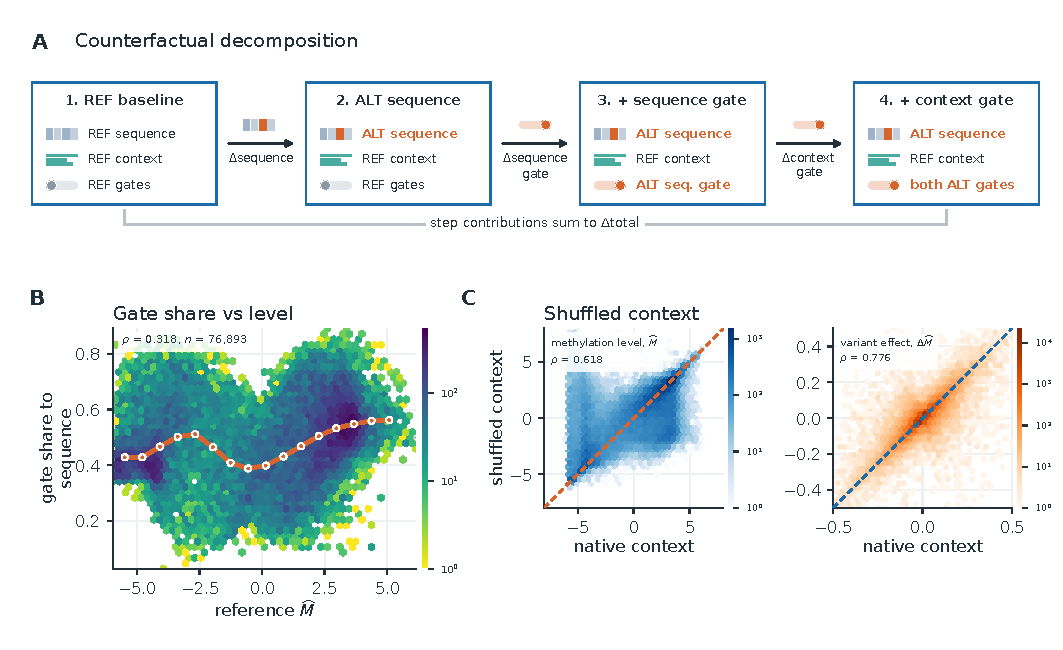
\includegraphics[width=\textwidth]{figures/fig4_context_mechanism.pdf}}{\figureplan{context mechanism}{a Paired model differences\quad b Counterfactual paths\\c Variance and partial correlation\quad d Context perturbation}}
\caption{\textbf{Context modulation and predictive information are distinct.}
\textbf{a}, Paired fusion-minus-sequence differences with 95\% block-bootstrap intervals.
\textbf{b}, Ordered counterfactual evaluations of the same fusion head separate sequence change, sequence-gate rescaling and context-gate rescaling.
\textbf{c}, Component-to-total variance ratios and gate-channel partial correlations. Covariance prevents variance ratios from summing to one.
\textbf{d}, Changes in predicted levels and effects under shuffled or median context, normalized to their unperturbed standard deviations. Decomposition and perturbation analyses use seed 42; they are distinct from the three-seed paired-model evaluation.}
\label{fig:context}
\end{figure*}

\subsection{Uncertainty and motif controls constrain interpretation}
Forward/reverse-complement disagreement provided a single-model indicator of unreliable locus predictions, with reported rank correlation near 0.50 against per-locus error. We compared it with variability across three training seeds, a boundary heuristic based on distance from predicted beta 0.5, and a random control. The boundary heuristic appeared especially informative on the beta scale, where predictions near zero or one can have compressed absolute errors. Its apparent advantage weakened on the unbounded $M$ scale and after stratification by predicted methylation (Supplementary Fig.~S1).

These comparisons support examining uncertainty-related scores on more than one scale. They do not demonstrate calibrated prediction intervals or make orientation disagreement a validated measure of error in a particular variant effect. Orientation averaging ensures invariant reported scores, while the disagreement before averaging remains a diagnostic of the underlying model. This distinction allows the same procedure to improve consistency without treating consistency as proof of biological accuracy.

Motif analyses provided another interpretation control. Across 831 JASPAR motifs, the strongest associations between motif-score change and predicted methylation response involved overlapping ETS matrices with the shared GGAA core. Motif weakening accompanied predicted hypermethylation, but the $k$-mer ridge reproduced these associations more strongly than the neural models. Overall disruption magnitude was unrelated to predicted effect ($\rho=-0.011$), and strongly disrupting variants did not show greater discrimination (Supplementary Fig.~S2). The evidence therefore supports sensitivity to sequence composition and motif-associated features, rather than establishing that the model learned transcription-factor binding grammar.

\subsection{Synonymous prioritization identifies an NCOA2 hypothesis}
We applied the paired scoring procedure to 440 synonymous SNV--CpG pairs on held-out chromosomes. Variants were ranked by the absolute predicted beta change using the current-context fusion model at seed 42. This screen asks which observed substitutions receive the largest local methylation responses, providing a practical starting point for selecting experiments. It is separate from the external mQTL and ASM evaluations, and cross-seed candidate stability has not yet been established for the current reference context.

Here, we use the dataset's top synonymous variant as an example of how an observed somatic change can be transformed into a biological hypothesis. chr8:g.70148394G$>$A in \textit{NCOA2} is a synonymous GGC$>$GGT substitution on transcript ENST00000452400.7. The variant is 9\,bp from probe cg20699548 and is located in the gene body. The probe has an OpenSea annotation and lies in the highest quartile of both ATAC-seq and H3K27ac signal. The current model predicted a hypomethylating shift of $\Delta\widehat\beta=-0.1539$ (Fig.~\ref{fig:candidates}a).

The \textit{NCOA2} candidate also had an extreme absolute response compared with a group of similar synonymous variants. Its predicted magnitude exceeded those of all 66 variants selected for the matched-background comparison (Fig.~\ref{fig:candidates}b). Matching makes the comparison more specific than placing the candidate against all substitutions, because the available background was selected for related mutation context and proximity. The result nevertheless describes the chosen observed comparator set, whose size and composition should remain visible alongside the candidate score. This establishes descriptive extremeness within that background, not a calibrated causal probability or a multiple-testing discovery. The candidate's short distance to its paired CpG is also relevant given the proximity effects in the external benchmarks.

Prioritized variants and associated genes can be investigated further to develop testable hypotheses. \textit{NCOA2} encodes a nuclear receptor coactivator, and previous work reported reduced breast-cancer cell proliferation after its depletion \cite{cai2019ncoa2}. That literature does not establish an effect of this substitution on cg20699548 or on gene expression. The present result instead motivates direct measurement of the CpG's methylation and \textit{NCOA2} expression following sequence perturbation. The locus's chromatin annotations describe its regulatory setting without independently validating the predicted mechanism.

\subsection{Nonsynonymous examples do not establish pathogenicity}
While the prioritization analysis focused on somatic synonymous variants, the framework extends to other single-nucleotide substitutions. Any scoreable base change can be introduced into the alternate sequence while reference context remains fixed, followed by the same orientation-averaged prediction difference. As an illustration, we evaluated nonsynonymous SNVs in breast-cancer-related genes. Two of the largest predicted responses were in \textit{STK11}, a gene associated with Peutz--Jeghers syndrome \cite{lipsa2019stk11}.

The variant rs2145420809, encoding p.Asn119Ser, was immediately adjacent to probe cg16601904 and produced predicted $\Delta\widehat\beta=0.0890$. Its probe lies at a CpG shelf, in the second ATAC-seq and third H3K27ac quartiles. The second example, rs148928808, encoding p.Tyr292Ter, was 205\,bp from cg08681293 and produced predicted $\Delta\widehat\beta=-0.0520$. That probe lies at a CpG shore, in the third ATAC-seq and second H3K27ac quartiles. Both variants are in the gene body on transcript NM\_000455.5 (Fig.~\ref{fig:candidates}c).

Both target probes belong to the training split. Their value is therefore to illustrate how variants can be placed within the complete scored background and selected for follow-up, not to provide independent validation. In particular, the established protein consequence of a truncating variant does not demonstrate that its predicted methylation response occurs experimentally or contributes to disease. The scoring framework measures a different proposed consequence that requires its own validation.

We tested this distinction more broadly using GWAS Catalog annotations. Among held-out pairs with measured methylation association, labeled and unlabeled variants were matched on distance and allele frequency. The GWAS fraction among the top 5\% of predicted effects was 0.510 (0.271--0.679) in eGTEx and 0.561 (0.402--0.728) in GENOA, without clear enrichment over the matched null (Fig.~\ref{fig:candidates}d). Predicted methylation-effect magnitude therefore did not provide a general classifier of disease annotation in these tests.

\begin{figure*}[t]
\centering
\IfFileExists{figures/fig5_variant_prioritization.pdf}{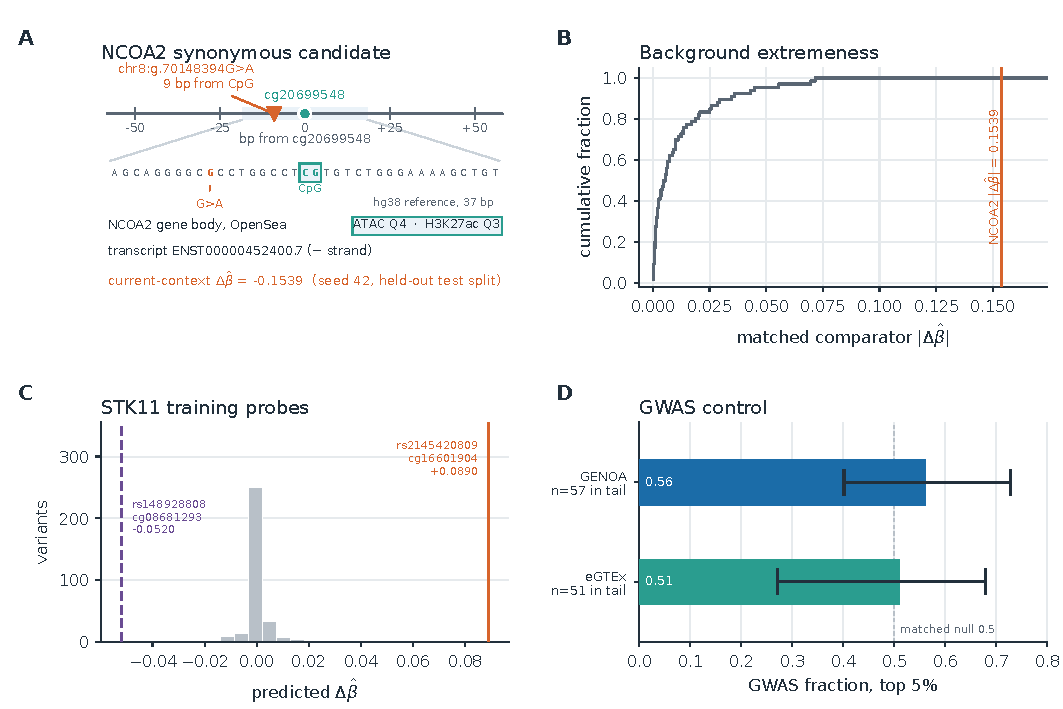
\includegraphics[width=\textwidth]{figures/fig5_variant_prioritization.pdf}}{\figureplan{variant prioritization}{a NCOA2 locus\quad b Matched background\\c STK11 examples\quad d GWAS enrichment control}}
\caption{\textbf{Predicted local methylation effects guide follow-up without establishing pathogenicity.}
\textbf{a}, The \textit{NCOA2} candidate and its nearby held-out CpG.
\textbf{b}, Its absolute predicted change compared with 66 matched synonymous variants; all scores use current-context seed 42.
\textbf{c}, Two \textit{STK11} examples in the nonsynonymous score distribution, explicitly labeled as training-probe applications.
\textbf{d}, GWAS-annotated fractions among the largest predicted effects in the distance- and frequency-matched GENOA cohort, at three tail depths, with 95\% 1-Mb block-bootstrap intervals and a matched null of 0.5. The eGTEx counterpart is omitted because no current-context export exists for it. Chromatin annotations describe loci and do not validate predicted mechanisms.}
\label{fig:candidates}
\end{figure*}

\section{Discussion}
SilentMethyl establishes a unified framework for two complementary tasks in regulatory genomics: predicting baseline CpG methylation and estimating how that methylation state responds to single-nucleotide variation. Across held-out chromosomes, integrating local DNA sequence with breast epigenomic context consistently improved methylation prediction over either modality alone. At the same time, paired REF--ALT scoring enabled the framework to prioritize individual variants according to their predicted local responses. The expanded evaluation shows why these tasks must nevertheless remain separate: the value of context for predicting an existing methylation state does not guarantee additional information about an allelic change.

The contribution of epigenomic context was particularly informative in accessible and H3K27ac-marked regulatory environments. CpG shores also showed substantial absolute improvement, although their relative gain was smaller than at islands. These observations are consistent with methylation reflecting both local sequence and regulatory state \cite{jones2012functions,schubeler2015function,encode2012integrated}. The H3K27me3 exception is equally relevant: some loci that transfer poorly across tissues receive relatively little benefit from the available reference context. The data therefore support complementary information from these modalities without a general rule that context rescues every sequence-model failure.

A distinct strength of the framework is that its variant-response predictions can be evaluated independently of baseline performance. Breast and blood mQTLs provide population-level evidence relating genotype to methylation, while ASM supplies a more direct allelic comparison within heterozygous samples. Agreement across these sources supports a real but modest predictive relationship. Lead-mQTL selection, observed-effect strength, distance and control-set construction all influence the apparent size of that relationship. Reporting these factors makes it possible to distinguish a successful positive control from performance over a broader set of candidate variants.

The distance analysis has practical consequences for model evaluation. A proximity gradient in predicted effects can be biologically plausible and still inflate discrimination when associated variants are closer to their CpGs than controls. Matching addresses this alternative explanation without requiring that all local effects have identical magnitude or range. The residual discrimination observed here is shared with other sequence-based architectures, so the contribution is a controlled characterization of variant prediction rather than a claim of universal superiority. Comparisons on common rows and negative sets are especially useful when marginal differences are small.

The gate decomposition further separates model sensitivity from useful predictive information. Identical context embeddings do not cancel from a nonlinear, sequence-dependent fusion model: changing an allele can change the gates and hence the contribution of reference context. Conversely, a sizable component of predicted-effect variance need not improve agreement with measured effects. The counterfactual decomposition documents this distinction for the fitted model, while its order dependence limits causal interpretation. Future architectures or context measurements may add allelic information, but that improvement should be established through external effect evaluation rather than inferred from better methylation-level accuracy.

The transfer analysis identifies another useful distinction between average performance and the loci most likely to need additional information. A small average penalty can coexist with concentrated errors at tissue-variable CpGs. These loci are informative targets for evaluating whether more representative reference measurements or tissue-specific training improve performance. Conversely, successful transfer at stable loci should not be generalized to regulatory regions with different methylation across tissues. Stratifying by measured variability makes that boundary visible without assuming that learned gate values reveal it.

The case studies retain the original practical objective of translating a prediction into a focused experimental question. For \textit{NCOA2}, proximity, a large predicted response and biological context identify a specific variant--CpG pair to investigate. For \textit{STK11}, the same procedure illustrates how a proposed epigenetic consequence can be considered alongside a protein-changing substitution. Neither example establishes that altered methylation mediates the variant's effect on expression or disease. Direct sequence perturbation, paired methylation measurement and assessment of expression would distinguish the predicted local response from the gene's broader biological relevance.

Several limitations define the scope of these findings. Methylation targets are cohort medians from 97 tumour-adjacent normal breast samples and may retain field effects and cell-composition heterogeneity \cite{tcga2012breast,teschendorff2016field}. Reference chromatin tracks are not matched individual epigenomes. The model consequently predicts a reference locus-level state rather than an individual's methylome. HM450 also samples only part of the genomic CpG space, and the ASM analysis evaluates positions outside that training distribution. Accuracy on these sites does not remove the need for broader coverage or independent breast-specific validation.

External germline associations do not directly validate the somatic synonymous screen. GENOA changes tissue, ancestry and study design together, so it cannot isolate ancestry-specific generalization. Predictions are limited to substitutions inside the local input window, leaving distal regulatory changes outside the model's scope. The current candidate screen uses one seed, making stability across training runs an outstanding requirement for individual rankings. Motif associations and GWAS overlap are also indirect endpoints; neither supplies a causal molecular mechanism. These constraints guide interpretation of the reported performance rather than being resolved by the number of evaluated pairs.

Together, the results show that sequence and reference chromatin can improve baseline methylation prediction while contributing differently to paired-allele inference. SilentMethyl provides a framework for evaluating that distinction and prioritizing local methylation hypotheses. Its strongest use is to narrow the set of variants and CpGs for direct investigation, with claims about effect magnitude, tissue specificity and disease relevance assessed separately.

\section{Methods}
\subsection{Data construction}
Methylation beta labels were constructed from the TCGA-BRCA HM450 matrix \cite{tcga2012breast,grossman2016gdc}. Using a sample-type-11 filter, 97 solid-tissue-normal columns were selected from 893 total. We checked that these 97 columns represented 97 unique participants without duplicate samples.

We represented single-probe methylation as the median of patient beta values. For CpG $i$, if $O_i$ represents the set of patients with a recorded methylation measurement at CpG $i$, then
\begin{gather*}
\beta_i=\operatorname{median}_{s\in O_i}\beta_{i,s},
\qquad y_i=\mathbf{1}[\beta_i>0.5],\\
\widetilde\beta_i=\max\left(10^{-4},\min\left(1-10^{-4},\beta_i\right)\right),\\
M_i=\log_2\left(\frac{\widetilde\beta_i}{1-\widetilde\beta_i}\right).
\end{gather*}
The transformation from beta to $M$-values follows \cite{du2010betamvalue}. The clipping prevents infinite regression targets at measured beta values of zero or one.

All probes required an exact CpG-centered DNA sequence and a valid reference context window. None of the 418,486 probes in the combined dataset were flagged by HM450's \texttt{MASK\_general} filter. Median probe coverage was 97 out of 97 samples, and 95.1\% of loci had at least 78 valid measurements. Probe coordinates and DNA sequence were taken from the hg38 HM450 annotation resource \cite{zhou2017infinium,chen2013crossreactive}.

The data were split by chromosome into training, validation, and test sets before model training. Chromosomes 10--11 formed the validation set, chromosomes 8--9 formed the test set, and the remaining chromosomes formed the training set. The corresponding locus counts were 345,359, 46,557 and 26,570. By separating data by chromosome, we ensured no sequence windows overlapped between training, validation, and testing sets. Three additional seed-42 evaluations used test chromosomes 12/18, 4/20 and 13/15/21. Partitions were disjoint within each evaluation; sex chromosomes remained in training and were not evaluated.

Each DNA input comprised a 1,000-bp CpG-centered sequence. The target CpG nucleotides were located at zero-indexed positions 499 and 500. The epigenetic input comprised seven primary breast-epithelium attributes: ATAC-seq chromatin accessibility and six histone marks (H3K4me3, H3K27ac, H3K27me3, H3K9me3, H3K36me3 and H3K4me1), averaged across a CpG-centered 100-bp window. Two PhyloP scores described the two central CpG nucleotides. A missingness mask accompanied each feature; missing values were imputed using the corresponding feature's global median. These reference data were derived from shared resources and were not patient-specific. Track accessions, checksums and build instructions are recorded in the reproduction documentation.

\subsection{Models and staged training}
The sequence module comprised a pretrained DNABERT-2 (117M) transformer \cite{zhou2024dnabert2}, followed by a convolutional layer. Masked attention pooling was then applied:
\[
\alpha_t=\frac{\exp(s_t)}{\sum_{u\in V}\exp(s_u)},\qquad
\mathbf h_{\rm seq}=\sum_{t\in V}\alpha_t\mathbf e_t,
\]
where $V$ contains non-padding positions and $\mathbf e_t$ denotes the embedding at position $t$. This produced a 768-dimensional sequence representation. The context component consisted of an MLP mapping the 18-dimensional reference input (nine features and nine masks) to a second 768-dimensional vector, $\mathbf h_{\rm ctx}$.

After LayerNorm, the two embeddings were concatenated into a 1,536-dimensional vector and passed through a gating MLP that produced $g_{\rm seq}$ and $g_{\rm ctx}$. The fused embedding was
\[
\mathbf z=g_{\rm seq}\widetilde{\mathbf h}_{\rm seq}
+g_{\rm ctx}\widetilde{\mathbf h}_{\rm ctx}.
\]
Two prediction heads used this embedding. The regression head predicted $M$, converted to beta by $\widehat\beta=2^{\widehat M}/(1+2^{\widehat M})$. The classification head produced a methylation probability, with the binary call defined by a threshold of 0.5. The training objective was the sum of Huber loss ($\delta=1.345$) on regression and binary cross-entropy on classification.

Sequence and context models were trained independently with AdamW, with DNABERT-2 fully fine-tuned. Sequence, context, and fusion training used up to 10, 15, and 10 epochs and learning rates of $2\times10^{-5}$, $10^{-3}$, and $5\times10^{-4}$, respectively. During fusion training, the component encoders were frozen and only the normalization, gating, and prediction modules were updated. Forward or reverse-complement DNA orientation was chosen with equal probability for each probe during training. For seeds 42, 43 and 44, the checkpoint was selected by lowest validation beta MAE.

Primary regression metrics included RMSE and MAE for both beta and $M$ values; classification was evaluated using ROC-AUC from continuous scores. CpGenie and DeepCpG were reimplemented from released source and trained on identical splits, windows, augmentation and loss, with validation-selected hyperparameters. DeepCpG used its DNA module because neighboring measured methylation does not change between paired alleles. Composition and reverse-complement-collapsed $k$-mer ridge models supplied simpler sequence baselines.

\subsection{Paired scoring and synonymous variant construction}
For each SNV, predicted methylation differences were calculated for both sequence orientations and then averaged:
\begin{align*}
\Delta\widehat\beta=\tfrac12\big[&\widehat\beta_{\mathrm{ALT,FWD}}-\widehat\beta_{\mathrm{REF,FWD}}\\
+&\widehat\beta_{\mathrm{ALT,RC}}-\widehat\beta_{\mathrm{REF,RC}}\big].
\end{align*}
$\Delta\widehat M$ was defined similarly. The reference context was held fixed between alleles. Averaging both orientations makes the reported score invariant under their interchange, whereas random orientation augmentation alone does not guarantee this property. For somatic candidates, REF and ALT correspond to the wild-type and mutated input sequences.

Tagged somatic synonymous SNVs were obtained through the GDC, and amino-acid preservation was verified using hg38 and GENCODE v44 \cite{grossman2016gdc,frankish2021gencode}. Variants were paired with the nearest HM450 probe. Filtering flagged probes and substitutions outside the probe's actual sequence window left 440 held-out candidate pairs. The current-context ranking uses seed 42 and absolute predicted beta change. Matched synonymous variants provided a descriptive background for individual responses. These comparisons are not a calibrated causal null or a basis for false-discovery claims. Nonsynonymous examples were processed through the same scoring procedure, with probe-split membership reported explicitly.

\subsection{External mQTL evaluation}
GENOA cis-meQTL summary statistics \cite{shang2023genoa} were converted from hg19 to hg38, checked against reference alleles and re-signed from minor-allele effects to the model's REF-to-ALT direction. Window and target-CpG filtering yielded 66,495 held-out pairs. Excluding CpG-creating or CpG-destroying changes left 42,866, including 4,037 significant pairs at $p<5\times10^{-8}$. eGTEx breast \cite{oliva2023mqtl} yielded 76,893 window-filtered pairs and 418 significant non-CpG-altering pairs under its study-specific permutation criterion (analysis cutoff $1.483\times10^{-5}$).

Signed Spearman correlation measured agreement in the relative ordering of signed responses. Direction agreement measured the proportion of predictions with the observed sign, and directional AUROC separated positive from negative observed effects using signed predictions. Absolute-effect correlations evaluated magnitude ordering. In contrast, discrimination AUROC used absolute predictions to separate associated from tested-but-null pairs. For distance-controlled discrimination, associated and control pairs were matched by variant--CpG distance; model comparisons used the same matched rows. The reproduction commands specify a 10-bp tolerance. Distance-only AUROC assessed residual imbalance.

Significant eGTEx breast lead mQTLs ($q<0.05$) were intersected with held-out CpGs. Removing variants outside the sequence window or altering the target CpG left 81 associations from 70 unique variants. A sensitivity analysis excluded variants overlapping or immediately adjacent to annotated probe spans. Significant and high-$q$ leads ($q\geq0.5$) were also matched on chromosome and allele frequency, requiring an MAF difference of at most 0.05 and preferring similar distance, baseline methylation and substitution type. This produced 35 pairs from pools of 53 significant and 51 high-$q$ variants. Pair resampling supplied confidence intervals, and within-pair label permutation supplied the discrimination test.

\subsection{Allele-specific methylation evaluation}
ASM pairs were drawn from the Rosenski--Dor--Kaplan and Do--Tycko catalogues, restricted to held-out chromosomes and CpGs inside the actual 1,000-bp model input. In Do--Tycko, predicted $\Delta\widehat M$ was averaged over each index SNP's scored DMR CpGs, yielding 722 SNP-level signed comparisons. Observed percentage-point differences and predicted $M$ differences were compared through sign, rank and directional AUROC, not direct magnitude calibration. Analyses used seed 42.

ASM discrimination used catalogue-specific controls: bimodal non-ASM loci for Rosenski and distance-matched non-DMR loci for Do--Tycko. Corresponding evaluation sets contained 6,910 and 10,746 rows. The latter catalogue's signed analysis used 179 1-Mb blocks; the Rosenski discrimination used 242. Recorded expectation bands were retained when assessing the primary result. Restriction to observed effects of at least 20 percentage points was post hoc. Full sample definitions and model-specific intervals are in Supplementary Table~S2.

\subsection{Transfer and gate decomposition}
Joint training allocated each probe to one tissue, preventing the same DNA window from carrying conflicting targets across tissues. The breast-held-out model excluded breast from both training and validation and was evaluated on the same breast test CpGs. Transfer error was related to measured cross-tissue variance, with and without adjustment for mean methylation. The comparison uses one held-out-tissue seed and a three-seed breast reference mean and does not isolate tissue from every training-design difference.

For the within-model decomposition, let $H$ denote the fitted regression head, $d_R,d_A$ the normalized REF/ALT sequence embeddings and $c$ the fixed normalized context embedding. The counterfactual representations were
\begin{align*}
z_R&=g_{d,R}d_R+g_{c,R}c,\\
z_S&=g_{d,R}d_A+g_{c,R}c,\\
z_D&=g_{d,A}d_A+g_{c,R}c,\\
z_A&=g_{d,A}d_A+g_{c,A}c.
\end{align*}
The differences $H(z_S)-H(z_R)$, $H(z_D)-H(z_S)$ and $H(z_A)-H(z_D)$ define the sequence, sequence-gate and context-gate components. Their sum equals the total contrast, including for nonlinear $H$. The final two form the gate channel. Components were calculated per orientation and averaged. Analyses used seed 42; partial rank correlations adjusted for the sequence channel. This ordered decomposition is not a unique causal attribution. Context perturbations compared identity, shuffled and median inputs, with deviations normalized by the unperturbed quantity's standard deviation.

\subsection{Statistical analysis and interpretation controls}
Confidence intervals generally resampled complete 1-Mb genomic blocks to preserve local dependence. Level-model paired comparisons used 5,000 replicates; context strata, primary cohort evaluation and ASM used 2,000; cross-cohort synthesis used 500; gate analyses used 1,000. Training-seed standard deviations and genomic-block intervals describe different sources of variation and were reported separately. Repeated chromosome partitions were fitted independently rather than pooled as independent participants.

Held-out CpGs were grouped by GENCODE region, CpG-island relation and chromatin-signal quartiles after model evaluation. Absolute context benefit was sequence-minus-fusion beta MAE; relative benefit divided that difference by sequence MAE. These annotations were used to interpret performance, not select checkpoints. Orientation disagreement was compared with seed variability, a boundary score $-|\widehat\beta-0.5|$ and a random control using risk--coverage curves and error correlations, repeated on beta and $M$ scales and within predicted-beta strata.

JASPAR motifs were scanned on both strands, with mutant scores evaluated at the same offset and strand as the best wild-type occurrence. Per-factor associations were corrected for multiple testing, with composition, distance and substitution controls. GWAS overlap was assigned by rsID or exact coordinate among held-out pairs with measured methylation association ($p<0.05$). Labeled and unlabeled variants were matched on distance and allele frequency, and genomic-block intervals assessed enrichment among the highest predicted effects. Supplementary analyses retain the associated sensitivity checks and source-data requirements.

\section*{Data availability}
The study uses public GDC, eGTEx, GENOA, ENCODE, GENCODE, UCSC and HM450 resources \cite{grossman2016gdc,oliva2023mqtl,shang2023genoa,encode2012integrated,frankish2021gencode,kent2002ucsc,zhou2017infinium}. Dataset identifiers, track accessions and checksums are recorded in the project reproduction documentation. Figure-level source-data tables should accompany the final submission.

\section*{Code availability}
The project repository is \url{https://github.com/ilikecheezits/SilentMethyl}. The supplied reproduction record describes model training, scoring, analysis and outstanding reruns. A versioned release identifier must be added before submission.

\IfFileExists{references.bib}{%
  {\small
  \setlength{\bibsep}{1pt plus 0.2ex}
  \bibliographystyle{unsrtnat}
  \bibliography{references}}
}{%
  {\small\noindent\textit{\texttt{references.bib} was not available when this
  draft was built, so citation keys are shown in place of formatted references.
  Building alongside the project bibliography restores the full list. Verify all entries against the project bibliography before submission.}\par\medskip}
  {\small
  \begin{thebibliography}{99}
\setlength{\itemsep}{2pt}
\bibitem{jones2012functions} \texttt{jones2012functions}
\bibitem{schubeler2015function} \texttt{schubeler2015function}
\bibitem{angermueller2017deepcpg} \texttt{angermueller2017deepcpg}
\bibitem{zhou2015predicting} \texttt{zhou2015predicting}
\bibitem{avsec2021effective} \texttt{avsec2021effective}
\bibitem{zeng2017cpgenie} \texttt{zeng2017cpgenie}
\bibitem{zhou2022interact} \texttt{zhou2022interact}
\bibitem{li2026deepmethylation} \texttt{li2026deepmethylation}
\bibitem{liu2025methven} \texttt{liu2025methven}
\bibitem{jin2026melody} \texttt{jin2026melody} --- Jin, Wang, Qiao \emph{et al.},
  ``Decoding the sequence determinants of locus-specific DNA methylation across
  human tissues,'' \emph{Nat. Commun.} (2026), doi:10.1038/s41467-026-76744-5.
\bibitem{mallet2021rc} \texttt{mallet2021rc}
\bibitem{sauna2011understanding} \texttt{sauna2011understanding}
\bibitem{stergachis2013exonic} \texttt{stergachis2013exonic}
\bibitem{alvarez2025mlh1} \texttt{alvarez2025mlh1}
\bibitem{blackburn2016tp53} \texttt{blackburn2016tp53}
\bibitem{jankowska2022adamts13} \texttt{jankowska2022adamts13}
\bibitem{cai2019ncoa2} \texttt{cai2019ncoa2}
\bibitem{lipsa2019stk11} \texttt{lipsa2019stk11}
\bibitem{encode2012integrated} \texttt{encode2012integrated}
\bibitem{tcga2012breast} \texttt{tcga2012breast}
\bibitem{teschendorff2016field} \texttt{teschendorff2016field}
\bibitem{grossman2016gdc} \texttt{grossman2016gdc}
\bibitem{du2010betamvalue} \texttt{du2010betamvalue}
\bibitem{zhou2017infinium} \texttt{zhou2017infinium}
\bibitem{chen2013crossreactive} \texttt{chen2013crossreactive}
\bibitem{zhou2024dnabert2} \texttt{zhou2024dnabert2}
\bibitem{frankish2021gencode} \texttt{frankish2021gencode}
\bibitem{shang2023genoa} \texttt{shang2023genoa}
\bibitem{oliva2023mqtl} \texttt{oliva2023mqtl}
\bibitem{kent2002ucsc} \texttt{kent2002ucsc}
\end{thebibliography}}
}


\end{document}
